\section {Systemarchitektur}
\author{Benjamin Besic}

\begin{figure}[htp]
    \centering
    \author{David Ignjatovic}
    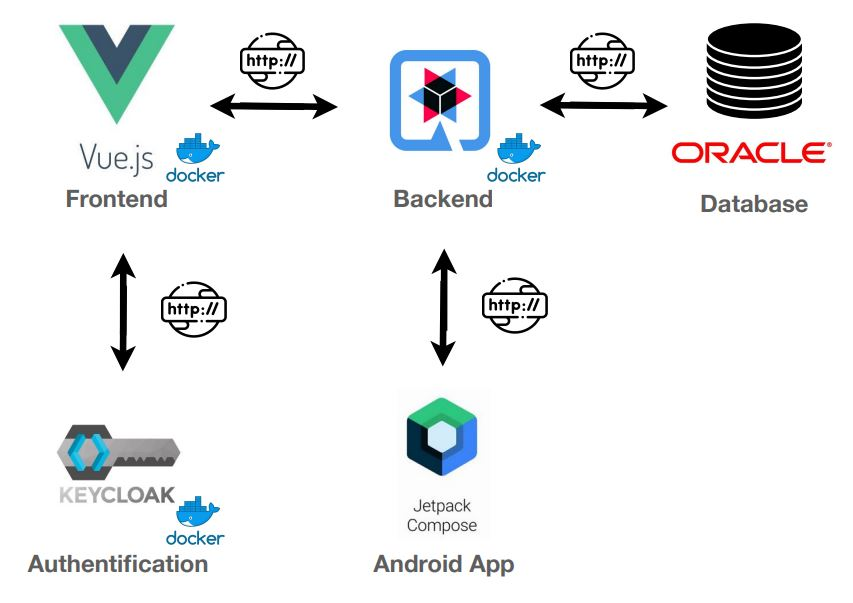
\includegraphics[scale=0.7]{pics/sys-arc-new.JPG}
    \caption{Systemarchitektur des Programms}
    \label{fig:impl:SysArc}
\end{figure}

\section{Datenmodell}
\author{David Ignjatovic}

Ein Datenmodell wird als Darstellung der relevanten Objekte eines Projektes verwendet. 
Unser Datenmodell ist im Großen und Ganzen immer gleichgeblieben. Für den Algorithmus aber haben wir es aber erweitern müssen.

\subsection{Entitäten}

Eine Entität ist ein bestimmtes Objekt mit den jeweiligen Atributen. Atribute sind die Eigenschaften eins Objektes.
Unser Projektes beinhaltet 5 Entitäten:

\begin{itemize}
  \item Bestellung
  \item Categories
  \item Kantine
  \item Menue
  \item Oeffungszeit
\end{itemize}

\texttt{Bestellung} 

Die Entität Bestellung enthält die wichtigsten Informationen über einen Mitarbeiter und die dazu ausgewählte Mahlzeit.
Zur Identifikation einer Bestellung verwenden wir eine Id welche generiert wird. \\*

In der Bestellung wird angegebebn von wem die Bestellung bestellt wurde und ob der Mitarbeiter es auch für sich selbst bestellt hat oder für jemand anderen. 
Jeder Mitarbeiter der Firma hat auch eine Personalnummer. Bei jeder Bestellung gibt es die möglichkeit einen Kommentar abzugeben. Dieser wird an die Kantine mitgegeben. Natürlich hat man auch die nöglichkeit 
eine Mahlzeit öfters zu bestellen. Somit hat jeder Mitarbeiter die möglichkeit eine Bestellanzahl mitzugeben. Für das bestellen, bearbeiten aber auch stonieren werden immer die jetztige uhrzeit mitgegeben. \\*

Das wichtigste in der Bestellung ist die Mahlzeit und für wann es bestellt wurde. Dafür verwenden wir die zwei klassen, Oeffnungszeit und Menue. \\*


\definecolor{dkgreen}{rgb}{0,0.6,0}
\definecolor{gray}{rgb}{0.5,0.5,0.5}
\definecolor{mauve}{rgb}{0.58,0,0.82}

\lstset{frame=tb,
  language=Java,
  aboveskip=3mm,
  belowskip=3mm,
  showstringspaces=false,
  columns=flexible,
  basicstyle={\small\ttfamily},
  numbers=none,
  numberstyle=\tiny\color{gray},
  keywordstyle=\color{blue},
  commentstyle=\color{dkgreen},
  stringstyle=\color{mauve},
  breaklines=true,
  breakatwhitespace=true,
  tabsize=3
}

\begin{lstlisting}
    @SequenceGenerator(name = "bestellung_seq_gen", sequenceName = "BESTELLUNG_SEQ",allocationSize=1)
    @GeneratedValue(strategy = GenerationType.SEQUENCE, generator = "bestellung_seq_gen")
    @Id
    @Column(name = "BESTELLUNG_ID")
    private Long id;

    @Column(name = "BESTELLTVON",length = 32)
    private String orderedBy;

    @Column(name = "BESTELLTFUER",length = 32)
    private String orderedFor;

    @Column(name = "KOMMENTAR",length = 4000)
    private String comment;

    @Column(name = "PERSONALNUMMER")
    private Long personalNumber;

    @Column(name = "ANZAHL")
    private int menueCounter;

    @Column(name = "STORNIERTUM",length = 6)
    private Timestamp canceledAt;

    @Column(name = "ABGERECHNETUM")
    private Timestamp settledAt;

    @Column(name = "KOSTENSTELLE")
    private Integer moneyPool;

    @Column(name = "ANGELEGTUM",length = 6)
    private Timestamp createdAt;

    @Column(name = "ANGELEGTVON",length = 32)
    private String createdBy;

    @Column(name = "GEAENDERTUM",length = 6)
    private Timestamp changedAt;

    @Column(name = "GEAENDERTVON",length = 32)
    private String changedBy;

    @ManyToOne
    @JoinColumn(name = "OEFFNUNGSZEIT_ID")
    private Oeffnungszeit oeffnungszeit;

    @ManyToOne
    @JoinColumn(name = "MENUE_ID")
    private Menue menue;
\end{lstlisting}

\texttt{Categories}

Die Entität Categories ist ein Enum, welches wir Hauptsächlich für unseren Algorithmus verwenden. Es besteht aus 4 einträgen: \\*


\begin{itemize}
    \item Vegetarisch
    \item Vegan
    \item Schwein
    \item Rind
    \item Huhn
    \item Pute
    \item Salat
    \item Nudel
    \item Süß
    \item Fisch
    \item Sonstiges
\end{itemize}

Die einzelnen Kategorien beschreiben eine Mahlezeit. Sommit kann man ganz einfach zwischen einzelnen Mahlezeiten unterscheiden und sie auch gruppieren.


\texttt{Kantine}



\section{REST-Schnittstellen}

\section{Authentifizierung}

\section {Interface Webapp}
\subsection{Login}
Beim Aufrufen der Webapp wird man zunächst zu der Login-Seite weitergeleitet. Wie diese fungiert, sieht man in der nächsten Abbildung. \\*
Der Login dient in erster Hinsicht dazu, um festzustellen ob der Benutzer ein Mitarbeiter oder Kantinenmitarbeiter ist.
Denn nach dem Login wird man entweder zur Mitarbeiter-Ansicht oder Kantinenmitarbeiter-Ansicht weitergeleitet. \\*
*Abbildung Login*

\subsection {Mitarbeiter-Ansicht}

\subsubsection {Home}
Das Erste, was ein Mitarbeiter zu sehen bekommt, ist die Home Ansicht. In dieser Ansicht ist eine Kalender und die Menüauswahl enthalten. \\*
Der Benutzer kann im Kalender das gewünschte Bestelldatum anklicken, dadurch wird automatisch die Menüauswahl aktualisiert. Man kann sich in die Zukunft, sowohl auch 
in die Vergangenheit klicken, um sich Auskunft über die vergangenen/kommenden Menüs zu beschaffen. Die Ansicht ist nur auf die Bestelltage beschränkt, an denen Menüs angeboten werden.\\*
Nach der erfolgreichen Datumswahl hat man unten drei Menüs zur Auswahl, sowohl wie die dazugehörige Vor- und Nachspeise. Das dem Benutzer empfohlene Menü (Analyse aus seinem Bestellverlauf) wird grün hinterlegt.
Neben den Bestellköpfen befindet sich ein Fragezeichen-Knopf, wenn man über diesen geht werden einem die Kategorien des Menüs angezeigt.
\\* Wenn die Bedingungen für eine Bestellung erfüllt sind,
kann man auf einen der drei Bestellknöpfe drücken, um zur Bestellansicht weitergeleitet zu werden. Sind diese Bedingungen nicht erfüllt, sind die Knöpfe ausgeschaltet. \\*
Weiters werden unter den Menüs noch relevante Informationen angezeigt. Durch das Klicken des Fragezeichen-Knopfs wird ein Bild der 14 Allergene geöffnet.

\begin{figure}[htp]
    \centering
    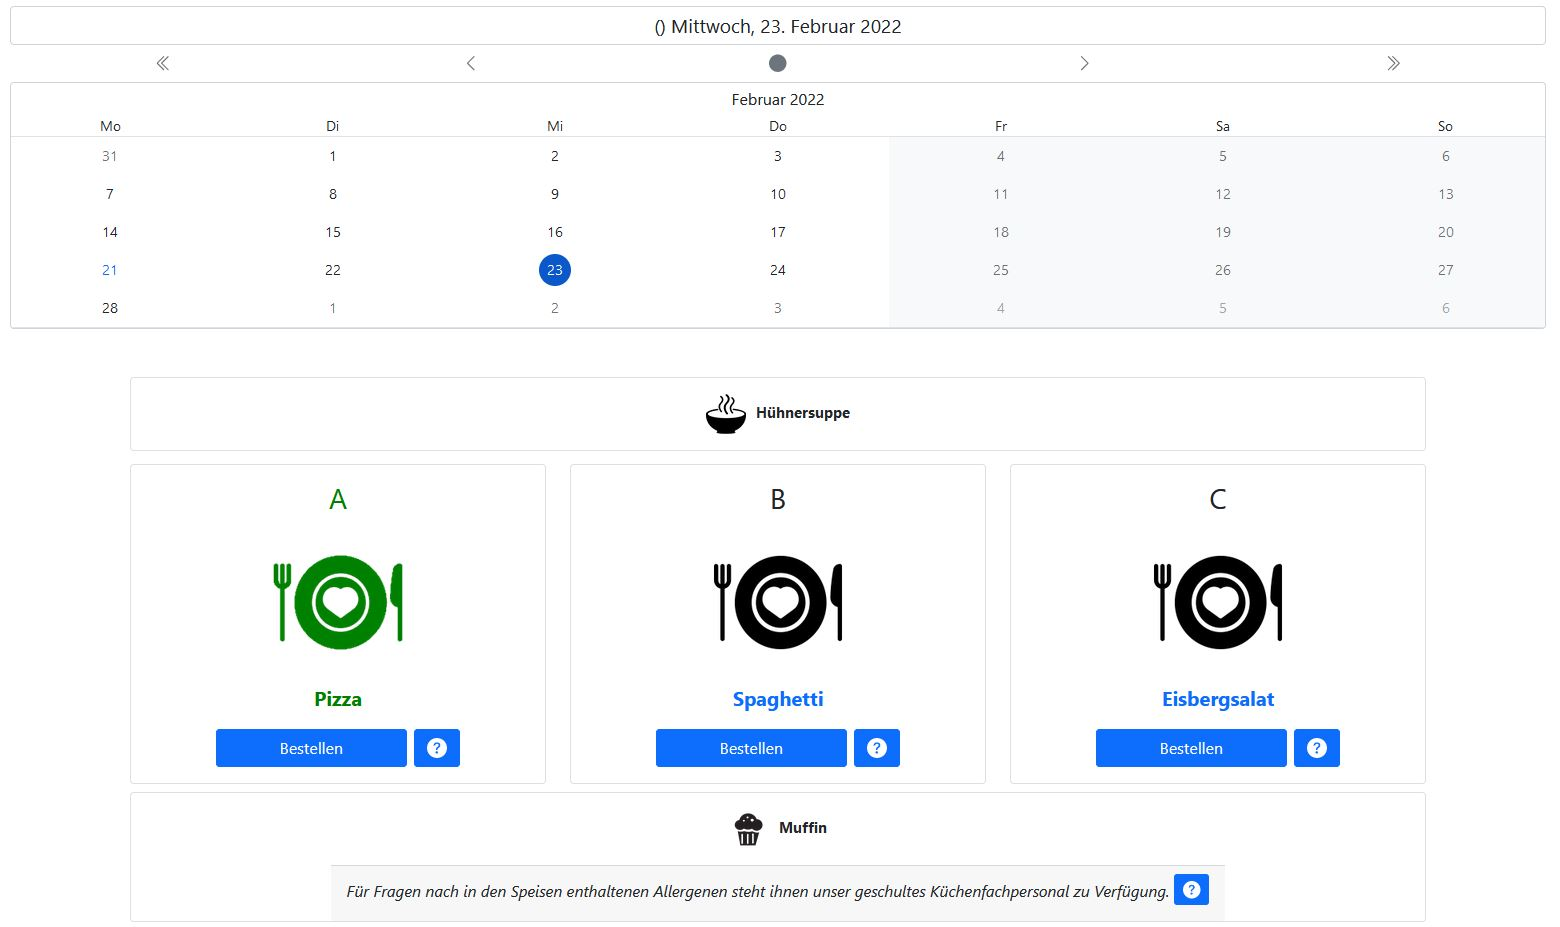
\includegraphics[scale=0.35]{pics/mitarbeiter-home.JPG}
    \caption{Home Ansicht eines Mitarbeiters}
    \label{fig:impl:HomeMitarbeiter}
\end{figure}

\pagebreak

\subsubsection {Bestellansicht}

In der Bestellansicht werden die nötigen Daten für die Bestellung ausgefüllt. Die ersten drei Felder sind automatisch ausgefüllt, aufgrund der vorherigen Auswahl. \\*
Die Tabelle auf der rechten Seite enthält alle Bestellzeiträume, die es gibt. Man kann nur eine gleichzeitig auswählen. Außerdem stehen die freien Plätze dabei, die aus der Datenbank geladen werden.\\*
Die Anzahl der Menüs kann durchs Klicken des Plus- und Minusknopfs angepasst werden.  \\*
Darunter steht voreingestellt der Benutzer, doch dies kann verändert werden, um das Menü für einen anderen Mitarbeiter bestellen zu können. \\*
Abschließend kann man noch einen Kommentar an die Kantine mitgeben, falls es etwaige Extrawünsche geben sollte. \\*
Die Bestellung kann durch den Abschließen-Knopf durchgeführt werden und Abbrechen kann man jederzeit mit dem Abbrechen-Knopf.
Die Bestellung ist erst ausführbar, sobald alle Felder außer des Kommentars ausgefüllt wurden.
\begin{figure}[htp]
    \centering
    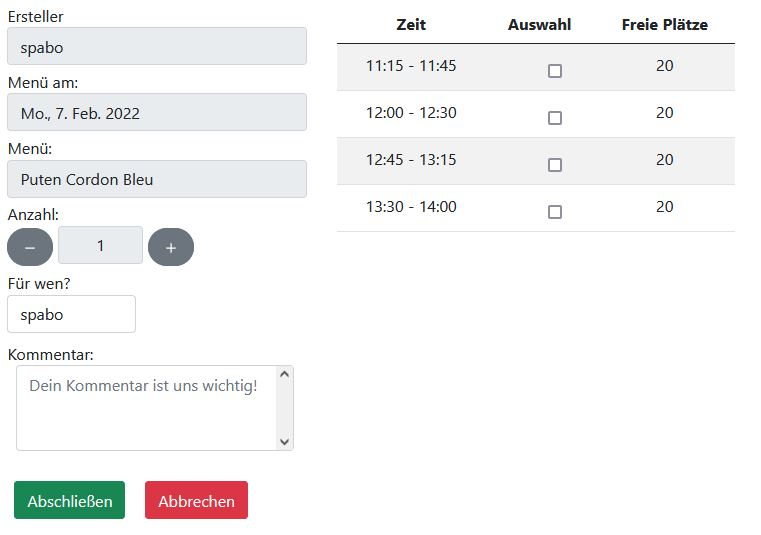
\includegraphics[scale=0.6]{pics/mitarbeiter-bestellen.JPG}
    \caption{Bestellansicht}
    \label{fig:impl:BestellenMitarbeiter}
\end{figure}
\pagebreak

\subsubsection {Bestellübersicht}

Die Bestellübersicht dient dem Benutzer dazu seine Bestellhistorie nachzuvollziehen. Zu jeder Bestellung ist der Name des bestellten Menüs, das Menüdatum, der Bestellzeitpunkt und die Essenszeit zugeordnet. \\*
Der Benutzer hat die Möglichkeit, oben in der Suchleiste, die Bestellungen nach Name oder Menüdatum zu filtern. Das Filtern erfolgt direkt nach der Eingabe. \\*
Man kann jede Bestellung anklicken und falls eine Bestellung die Stornierbedingungen erfüllt kann diese mit dem unten gelegen Storno-Button storniert werden.
Nach einer erfolgreichen Stornierung verschwindet die Bestellung aus dem Verlauf, doch in der Datenbank wird nur das Stornierdatum gesetzt und somit wird die Bestellung ungültig gemacht. 


\begin{figure}[htp]
    \centering
    \includegraphics[scale=0.4]{pics/mitarbeiter-bestellen-übersicht.JPG}
    \caption{Bestellungsübersicht}
    \label{fig:impl:BestellenMitarbeiterUebersicht}
\end{figure}
\pagebreak

\subsubsection {Statistiken}

Der Benutzer kann in dieser Ansicht mehr Informationen über seine vergangenen Bestellungen bekommen.
Durch das Wechseln des Tabs oben links wird entweder eine Statistik über die Kategorien oder über die Wochentage angezeigt.

\begin{figure}[htp]
    \centering
    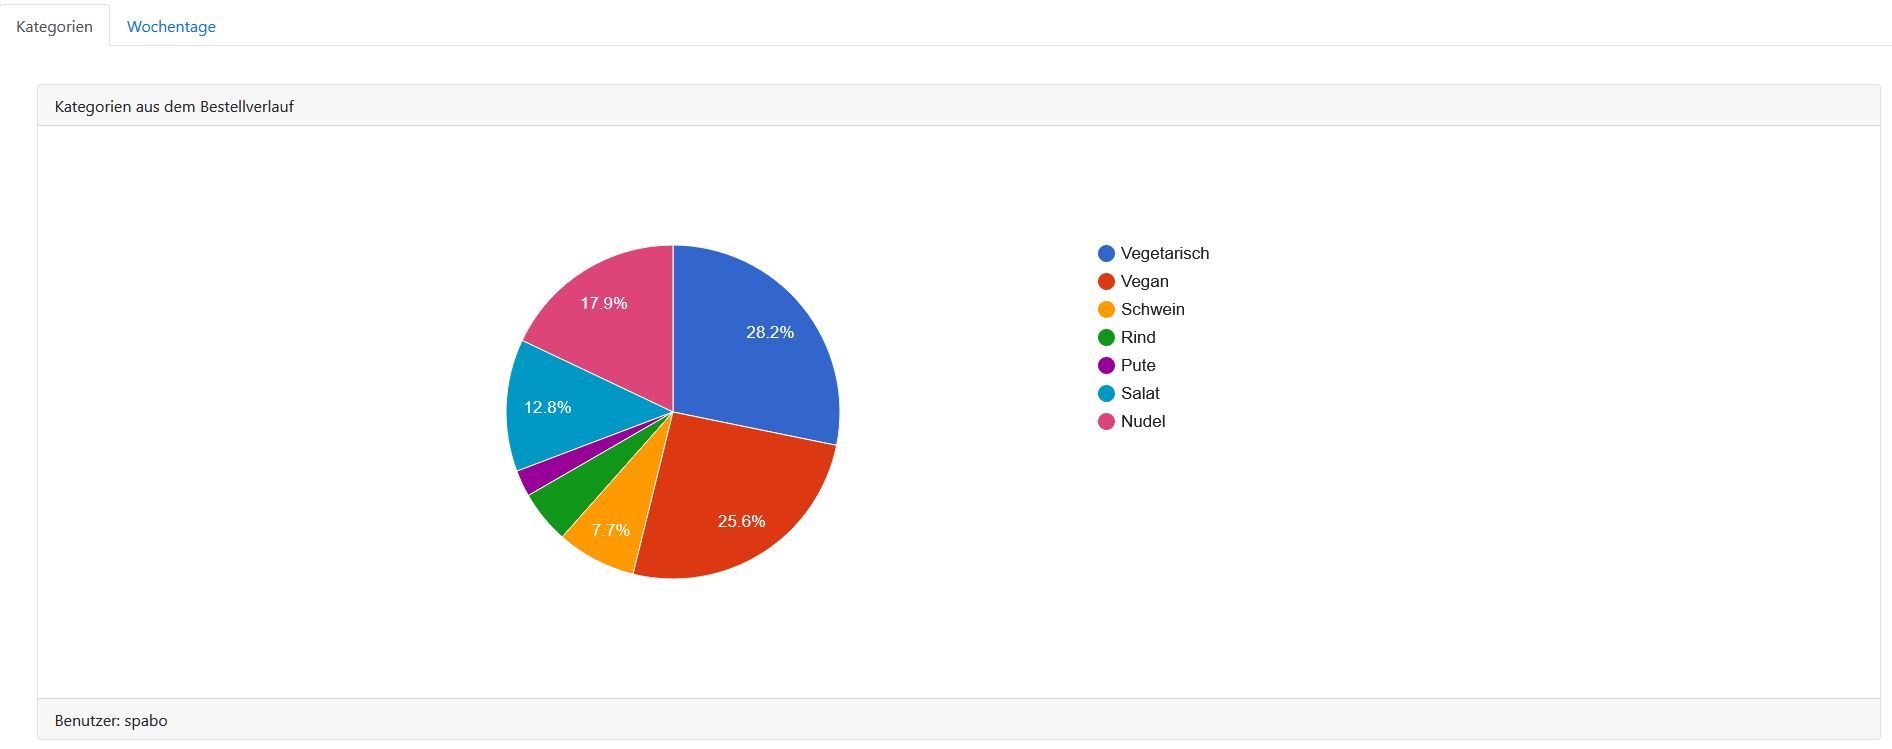
\includegraphics[scale=0.3]{pics/statistiken_kategorien.JPG}
    \caption{Kategorie Statistiken}
    \label{fig:impl:StatsCategories}
\end{figure}

\begin{figure}[htp]
    \centering
    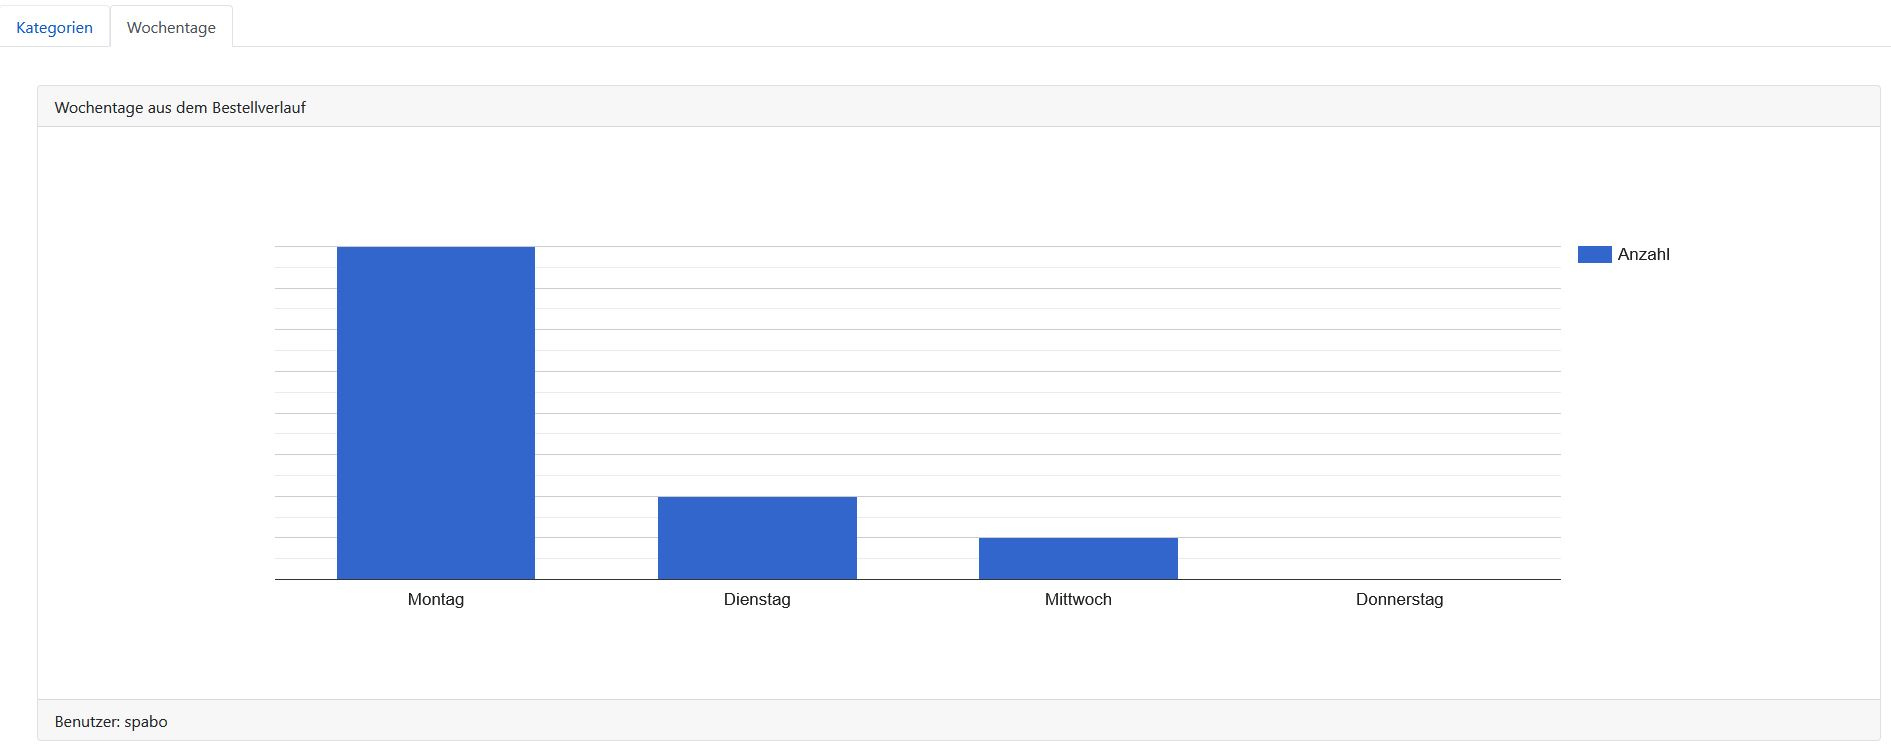
\includegraphics[scale=0.3]{pics/statistiken_wochentage.JPG}
    \caption{Wochentage Statistiken}
    \label{fig:impl:WeekDaysCategories}
\end{figure}

\pagebreak

\subsection {Kantinen-Ansicht}
\subsubsection {Home}
\subsubsection {Drucken}

\section {Interface Android-App}

